\chapter{Ultrasonido}
\subsection{Objetivo}
Implementar un circuito capaz de hacer mediciones de distancia con un sensor ultrasonico HC-SR04 (diseñado para ser usado en Arduino) sin el uso de ningún tipo de logica programable.
\subsection{Analisis}
Para poder empezar con el proceso de diseño se analizaron todas las etapas por las que deberian viajar las señales con el fin de realizar lo pedido.
\begin{center}

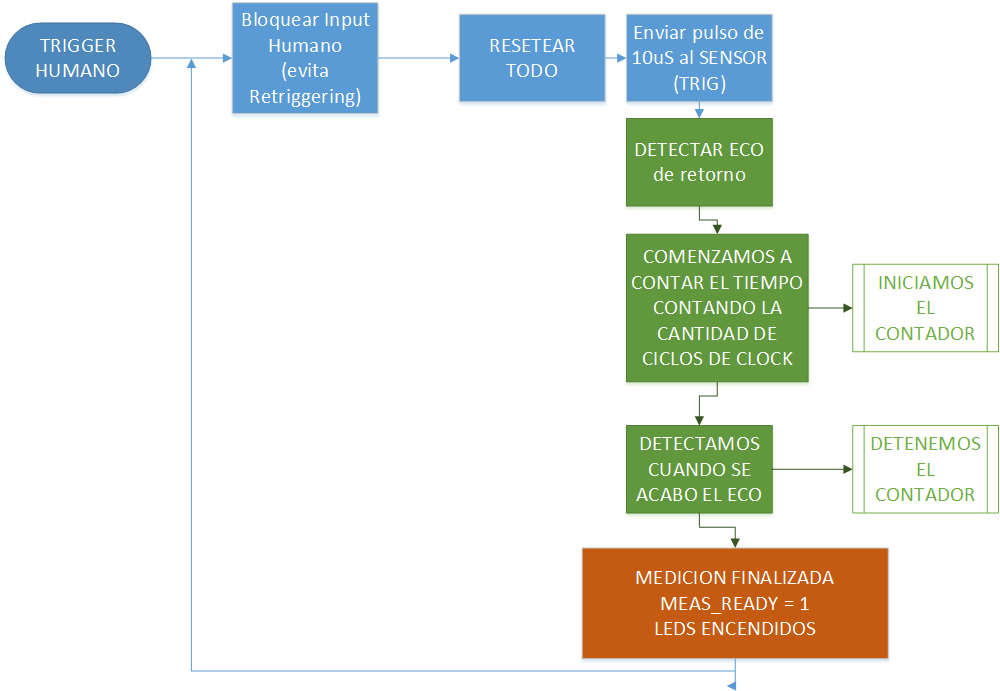
\includegraphics[scale=0.5,keepaspectratio]{../8-UltraSound/Driagrama-de-Flujo.png}

\end{center}
El diseño comienza por la construcción de un sistema de trigger que permita los procesos siguientes.
Para dicho sistema se podria haber optado por la implementación de un pulsador 